\documentclass[12pt,a4paper]{article}
\usepackage[utf8]{inputenc}
\usepackage[T2A]{fontenc}
\usepackage[russian]{babel}
\usepackage{amsmath, amssymb}
\usepackage{geometry}
\usepackage{graphicx}
\usepackage{booktabs}
\usepackage{array}
\usepackage{float}
\usepackage{hyperref}
\geometry{left=2.5cm, right=2cm, top=2cm, bottom=2cm}


\begin{document}
	
	%--- Титульная страница ---%
	\thispagestyle{empty}
	\begin{titlepage}
		\begin{center}
			\textbf{МИНИСТЕРСТВО НАУКИ И ВЫСШЕГО ОБРАЗОВАНИЯ\\
				РОССИЙСКОЙ ФЕДЕРАЦИИ}\\[6pt]
			Федеральное государственное автономное образовательное учреждение\\
			высшего образования <<Санкт-Петербургский политехнический\\
			университет Петра Великого>>\\[6pt]
			Институт компьютерных наук и кибербезопасности\\
			Высшая школа технологий искусственного интеллекта\\[6pt]
			Направление: 02.03.01 <<Математика и компьютерные науки>>
			
			\vfill
			
			{\large\textbf{Индивидуальное домашнее задание №4}}\\[6pt]
			по дисциплине\\[4pt]
			{\large <<Математическая статистика>>}\\[12pt]
			{\large Вариант №{} 14}
			
			\vfill
			
			\small{
				\begin{tabular}{lrrl}
					\!\!\!Студент, & \hspace{2cm} & & \\
					\!\!\!группы 5130201/30102 & \hspace{2cm} & \underline{\hspace{3cm}} & Санько В. В. \\\\
					\!\!\!Преподаватель & \hspace{2cm} & \underline{\hspace{3cm}} & Малов С. В. \\\\
					&&\hspace{4cm}
				\end{tabular}
				\begin{flushright}
					<<\underline{\hspace{1cm}}>>\underline{\hspace{2.5cm}} 2026 г.
				\end{flushright}
			}
			
			\hfill\break
			\begin{center}\small{Санкт-Петербург, 2026}\end{center}
		\end{center}
	\end{titlepage}


\newpage
\setcounter{page}{2}
%=============================================================
\section{Часть 1. Регрессионный анализ}
%=============================================================

\subsection*{Данные}

Параметры: $\alpha = 0.10$, $h = 1.80$.

\[
Y = (11.83,\, 15.46,\, 18.12,\, \ldots,\, 14.84,\, 13.92), \quad n = 50
\]
\[
X = (3,\, 2,\, 1,\, 3,\, 1,\, 3,\, 1,\, 3,\, \ldots,\, 1,\, 2), \quad X \in \{0,1,2,3\}
\]

%-------------------------------------------------------------
\subsection{Задание A. Линейная регрессионная модель}
%-------------------------------------------------------------

Линейная регрессионная модель имеет вид:
\[
Y = \beta_1 + \beta_2 X + \varepsilon, \quad \varepsilon \sim N(0, \sigma^2).
\]

Матрица плана $\mathbf{X}_l$ размера $2 \times 50$; МНК-оценка параметров:
\[
\hat{\boldsymbol{\beta}} = \bigl(\mathbf{X}_l \mathbf{X}_l^\top\bigr)^{-1} \mathbf{X}_l \mathbf{Y}.
\]

\textbf{МНК-оценки:}
\[
\hat{\beta}_1 = 15{,}6865, \qquad \hat{\beta}_2 = -0{,}3474.
\]

Построенная линия регрессии: $\hat{Y} = 15{,}6865 - 0{,}3474\, X$.

\begin{figure}[H]
  \centering
  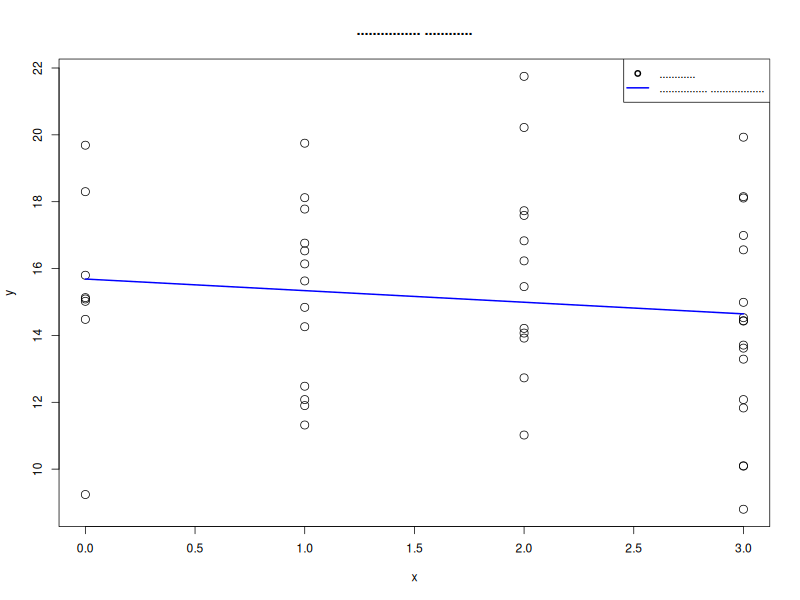
\includegraphics[width=0.75\textwidth]{plot_A_linear.png}
  \caption{Линейная регрессионная модель. Синяя линия~--- оценка МНК.}
\end{figure}

\textit{Визуальная оценка:} разброс точек значителен, линия почти горизонтальна, что указывает на слабую линейную зависимость $Y$ от $X$.

%-------------------------------------------------------------
\subsection{Задание B. Полиномиальная модель}
%-------------------------------------------------------------

Добавим квадратичный член:
\[
Y = \beta_1 + \beta_2 X + \beta_3 X^2 + \varepsilon.
\]

Матрица плана $\mathbf{X}$ размера $3 \times 50$; МНК-оценка:
\[
\hat{\boldsymbol{\beta}} = \bigl(\mathbf{X}\mathbf{X}^\top\bigr)^{-1}\mathbf{X}\mathbf{Y}.
\]

\textbf{МНК-оценки полиномиальной модели:}
\[
\hat{\beta}_1 = 15{,}0769, \qquad
\hat{\beta}_2 = 1{,}0452, \qquad
\hat{\beta}_3 = -0{,}4302.
\]

\begin{figure}[H]
  \centering
  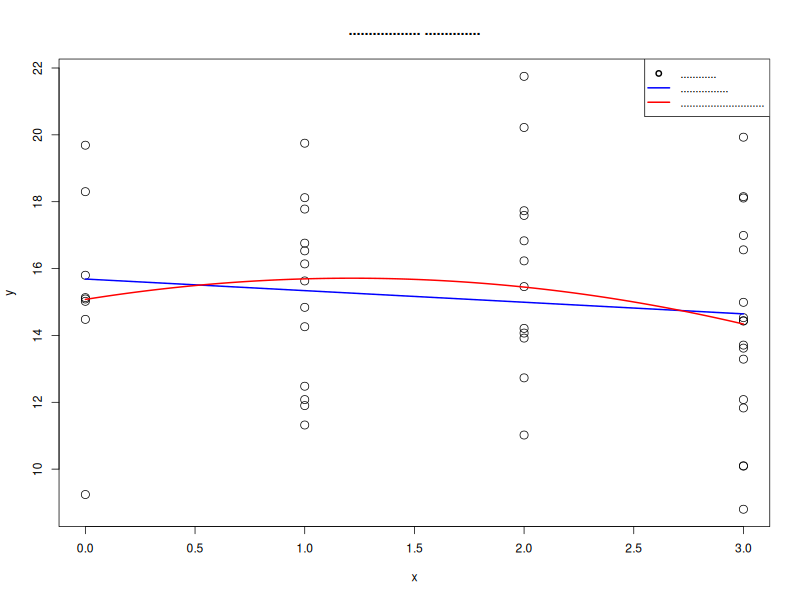
\includegraphics[width=0.75\textwidth]{plot_B_poly.png}
  \caption{Сравнение моделей: синяя~--- линейная, красная~--- квадратичная.}
\end{figure}

\textit{Визуальная оценка:} обе кривые близки между собой, разброс точек велик. Квадратичный член незначительно улучшает подгонку.

%-------------------------------------------------------------
\subsection{Задание C. Гистограмма остатков. Проверка нормальности}
%-------------------------------------------------------------

Остатки полиномиальной модели: $\hat{\varepsilon} = \mathbf{Y} - \mathbf{X}^\top\hat{\boldsymbol{\beta}}$.

\textbf{Параметры гистограммы} (шаг $h = 1{,}80$):
\begin{center}
\begin{tabular}{lrrrrrrr}
\toprule
Границы & $-5{,}84$ & $-4{,}04$ & $-2{,}24$ & $-0{,}44$ & $1{,}36$ & $3{,}16$ & $4{,}96$ \\
\midrule
Частоты & 6 & 6 & 9 & 14 & 7 & 6 & 2 \\
\bottomrule
\end{tabular}
\end{center}

\begin{figure}[H]
  \centering
  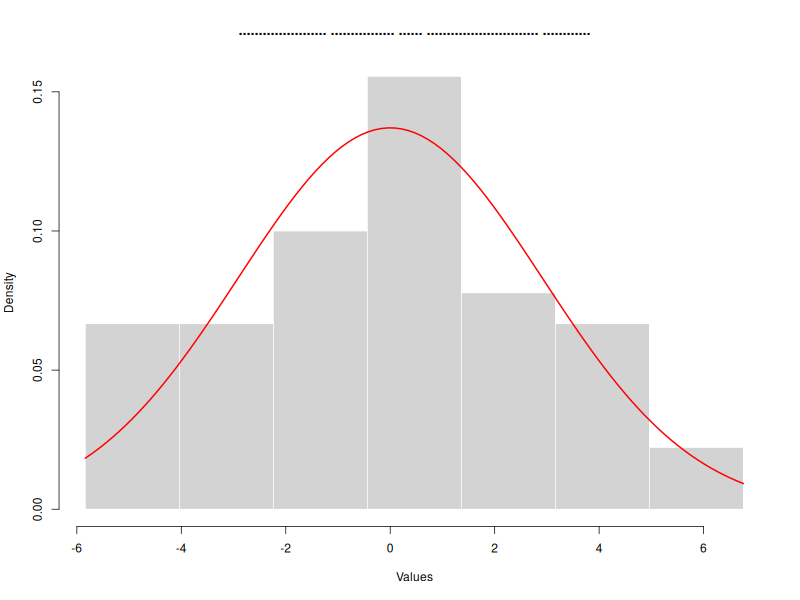
\includegraphics[width=0.75\textwidth]{plot_C_hist.png}
  \caption{Гистограмма остатков. Красная кривая~--- плотность $N(0, s^2)$.}
\end{figure}

\textbf{Тест $\chi^2$ на нормальность} (сложная гипотеза, оцениваем $\sigma$, $k=7$, $\nu = k-1-1 = 5$):
\[
X^2 = 3{,}2804, \qquad \chi^2_{5;\, 0{,}90} = 9{,}2364, \qquad \text{P-значение} = 0{,}6568.
\]

Поскольку $X^2 = 3{,}28 < \chi^2_{5;\, 0{,}90} = 9{,}24$, \textbf{гипотеза о нормальности остатков принимается} на уровне значимости $\alpha = 0{,}10$.

%-------------------------------------------------------------
\subsection{Задание D. Доверительные интервалы для $\beta_2$ и $\beta_3$}
%-------------------------------------------------------------

При предположении нормальности ошибок и уровне доверия $1 - \alpha = 0{,}90$ строим частные доверительные интервалы:

\begin{center}
\begin{tabular}{lccc}
\toprule
Параметр & Оценка & Нижняя граница & Верхняя граница \\
\midrule
$\beta_1$ & $15{,}0769$ & $13{,}3829$ & $16{,}7710$ \\
$\beta_2$ & $1{,}0452$  & $-1{,}4047$ & $3{,}4951$  \\
$\beta_3$ & $-0{,}4302$ & $-1{,}1601$ & $0{,}2996$  \\
\bottomrule
\end{tabular}
\end{center}

\textit{Интерпретация:}
\begin{itemize}
  \item $\beta_1$: интервал $[13{,}38;\, 16{,}77]$ не содержит нуль~--- параметр \textbf{значим}.
  \item $\beta_2$: интервал $[-1{,}40;\, 3{,}50]$ содержит нуль~--- линейный эффект \textbf{не значим}.
  \item $\beta_3$: интервал $[-1{,}16;\, 0{,}30]$ содержит нуль~--- квадратичный эффект \textbf{не значим}.
\end{itemize}

%-------------------------------------------------------------
\subsection{Задание E. Гипотезы линейности и независимости}
%-------------------------------------------------------------

\paragraph{Гипотеза линейности.} $H_0: \beta_3 = 0$ (квадратичная зависимость сводится к линейной).

Функционал $\psi = (0\; 0\; 1)\boldsymbol{\beta} = \beta_3$, размерность $q = 1$.
\[
F = \frac{(\mathbf{C}\hat{\boldsymbol{\beta}})^\top\bigl[s^2\,\mathbf{C}(\mathbf{X}\mathbf{X}^\top)^{-1}\mathbf{C}^\top\bigr]^{-1}(\mathbf{C}\hat{\boldsymbol{\beta}})}{q}
  = 0{,}9783, \qquad F_{1,\,47;\,0{,}90} = 2{,}8154.
\]
$F = 0{,}98 < 2{,}82$~--- \textbf{гипотеза линейности принимается} (P-значение $= 0{,}328$).

\paragraph{Гипотеза независимости.} $H_0: \beta_2 = 0,\; \beta_3 = 0$ ($Y$ не зависит от $X$).

Функционал $\psi = \begin{pmatrix}0&1&0\\0&0&1\end{pmatrix}\boldsymbol{\beta}$, размерность $q = 2$.
\[
F = 0{,}8931, \qquad F_{2,\,47;\,0{,}90} = 2{,}4192.
\]
$F = 0{,}89 < 2{,}42$~--- \textbf{гипотеза независимости принимается} (P-значение $= 0{,}416$).

%-------------------------------------------------------------
\subsection{Задание F. Выбор наилучшей модели (AIC и BIC)}
%-------------------------------------------------------------

Рассматриваем три модели:
\begin{itemize}
  \item Модель~(1): $E(Y\mid X) = \beta_1 + \beta_2 X$ (линейная),
  \item Модель~(2): $E(Y\mid X) = \beta_1 + \beta_2 X + \beta_3 X^2$ (квадратичная),
  \item Модель~(3): $E(Y) = \beta_1$ (константа, независимость от $X$).
\end{itemize}

\begin{center}
\begin{tabular}{lccc}
\toprule
Модель & Число параметров & AIC & BIC \\
\midrule
(1) Линейная     & 3 & $254{,}76$ & $260{,}49$ \\
(2) Квадратичная & 4 & $255{,}73$ & $263{,}38$ \\
(3) Константа    & 2 & $\mathbf{253{,}59}$ & $\mathbf{257{,}42}$ \\
\bottomrule
\end{tabular}
\end{center}

По обоим критериям наилучшей оказалась \textbf{модель~(3) --- константа}.

%-------------------------------------------------------------
\subsection{Задание G. Интерпретация результатов}
%-------------------------------------------------------------

\begin{enumerate}
  \item Линейная модель: $\hat{Y} = 15{,}69 - 0{,}35\,X$. Коэффициент $\hat{\beta}_2 = -0{,}35$ незначим.
  \item Квадратичная модель: $\hat{Y} = 15{,}08 + 1{,}05\,X - 0{,}43\,X^2$. Оба коэффициента при $X$ и $X^2$ незначимы.
  \item Остатки квадратичной модели \textbf{нормально распределены} (тест $\chi^2$ принят).
  \item Нет статистических оснований утверждать нелинейность зависимости (тест на линейность принят).
  \item Нет статистических оснований утверждать зависимость $Y$ от $X$ (тест на независимость принят).
  \item По критериям AIC и BIC наилучшая модель~--- \textbf{константа}: $E(Y) = \beta_1$. Это согласуется с результатами тестов~E.
  \item \textbf{Вывод:} в данном наборе данных ковариата $X$ не оказывает статистически значимого влияния на $Y$.
\end{enumerate}

\newpage
%=============================================================
\section{Часть 2. Двухфакторный дисперсионный анализ}
%=============================================================

\subsection*{Данные}

Параметры: $\alpha_1 = 0{,}01$, $h = 1{,}40$.
Число наблюдений $n = 40$, факторы $A$ ($d_1 = 5$ уровней) и $B$ ($d_2 = 4$ уровня).

%-------------------------------------------------------------
\subsection{Задание A. Двухфакторная модель. МНК-оценки}
%-------------------------------------------------------------

Полная модель с взаимодействием:
\[
Y_{ijk} = \mu_{ij} + \varepsilon_{ijk},
\quad \varepsilon_{ijk} \overset{\text{i.i.d.}}{\sim} N(0, \sigma^2),
\]
где $\mu_{ij} = \mu + \alpha_i + \beta_j + (\alpha\beta)_{ij}$, $i=1,\ldots,5$; $j=1,\ldots,4$.

МНК-оценка через индикаторную матрицу $\mathbf{X}_M$ ($20 \times 40$):
\[
\hat{\boldsymbol{\mu}} = (\mathbf{X}_M \mathbf{X}_M^\top)^{-1} \mathbf{X}_M \mathbf{Y}.
\]

\textbf{Несмещённая оценка дисперсии:}
\[
s^2 = \frac{\text{SSE}}{n - d_1 d_2} = \frac{61{,}23}{40 - 20} = 3{,}0615.
\]

Ячеечные средние $\hat{\mu}_{ij}$ (строки~--- уровни $A$, столбцы~--- уровни $B$):

\begin{center}
\begin{tabular}{ccccc}
\toprule
 & $B=1$ & $B=2$ & $B=3$ & $B=4$ \\
\midrule
$A=1$ & $19{,}44$ & $20{,}39$ & $16{,}02$ & $16{,}75$ \\
$A=2$ & $19{,}75$ & $20{,}11$ & $14{,}67$ & $14{,}80$ \\
$A=3$ & $20{,}87$ & $21{,}24$ & $15{,}45$ & $16{,}80$ \\
$A=4$ & $18{,}08$ & $18{,}87$ & $13{,}72$ & $14{,}52$ \\
$A=5$ & --- & $17{,}84$ & $10{,}36$ & $13{,}51$ \\
\bottomrule
\end{tabular}
\end{center}

%-------------------------------------------------------------
\subsection{Задание B. Аддитивность. График взаимодействия}
%-------------------------------------------------------------

\begin{figure}[H]
  \centering
  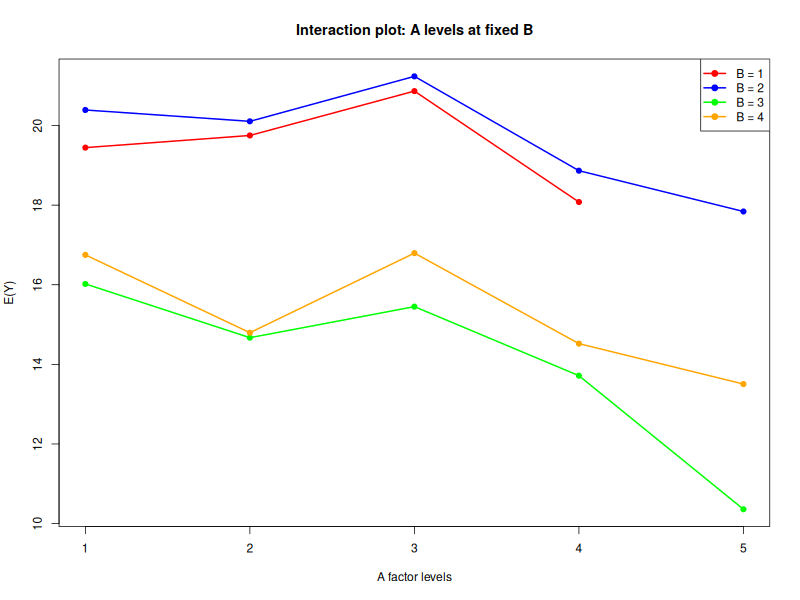
\includegraphics[width=0.75\textwidth]{plot2_B_interaction.png}
  \caption{Зависимость $\hat{\mu}_{ij}$ от уровней фактора $A$ при каждом фиксированном $B$.}
\end{figure}

\textbf{Проверка взаимодействия:} ANOVA для полной модели:

\begin{center}
\begin{tabular}{lrrrrr}
\toprule
Источник & SS & Df & MS & $F$ & P-значение \\
\midrule
$A$      & $90{,}27$  & 4  & $22{,}57$ & $7{,}74$ & $0{,}0005$ \\
$B$      & $221{,}53$ & 3  & $73{,}84$ & $25{,}33$ & $< 10^{-6}$ \\
$A:B$    & $10{,}17$  & 11 & $0{,}92$  & $0{,}32$ & $0{,}9733$ \\
Residuals & $61{,}23$ & 21 & $2{,}92$  & & \\
\bottomrule
\end{tabular}
\end{center}

P-значение для взаимодействия $A:B$ равно $0{,}9733 \gg 0{,}01$~--- \textbf{взаимодействие не значимо}. На графике линии почти параллельны, что визуально подтверждает \textbf{аддитивность} модели.

%-------------------------------------------------------------
\subsection{Задание C. Анализ остатков. Нормальность}
%-------------------------------------------------------------

\begin{figure}[H]
  \centering
  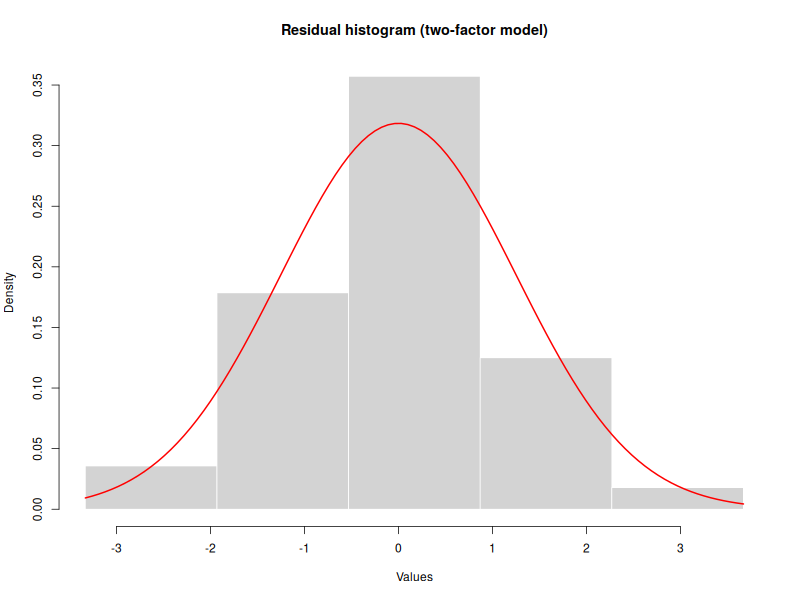
\includegraphics[width=0.75\textwidth]{plot2_C_hist.png}
  \caption{Гистограмма остатков двухфакторной модели (шаг $h = 1{,}40$).}
\end{figure}

\textbf{Параметры гистограммы:}
\begin{center}
\begin{tabular}{lrrrrrr}
\toprule
Границы & $-3{,}33$ & $-1{,}93$ & $-0{,}53$ & $0{,}87$ & $2{,}27$ & $3{,}67$ \\
\midrule
Частоты & 2 & 10 & 20 & 7 & 1 & \\
\bottomrule
\end{tabular}
\end{center}

\textbf{Тест $\chi^2$} ($k = 5$, $\nu = k-1-1 = 3$):
\[
X^2 = 0{,}4237, \qquad \chi^2_{3;\, 0{,}99} = 11{,}3449, \qquad \text{P-значение} = 0{,}9353.
\]

$X^2 = 0{,}42 \ll \chi^2_{3;\, 0{,}99} = 11{,}34$~--- \textbf{гипотеза о нормальности принимается} на уровне $\alpha_1 = 0{,}01$.

%-------------------------------------------------------------
\subsection{Задание D. Дисперсионный анализ}
%-------------------------------------------------------------

Сравниваем вложенные модели с полной $q$ (со взаимодействием). Остаточные степени свободы полной модели: $r = n - d_1 d_2 = 20$.

\begin{center}
\begin{tabular}{lrrrrrr}
\toprule
Гипотеза & SS$_H$ & Df$_H$ & MS$_H$ & $F$ & $F_{\alpha_1}$ & P-знач. \\
\midrule
$H_{12}$: нет $A\!:\!B$   & $10{,}17$  & 11 & $0{,}92$  & $0{,}317$  & $3{,}294$ & $0{,}973$ \\
$H_1$: нет $A$             & $82{,}34$  & 15 & $5{,}49$  & $1{,}883$  & $3{,}088$ & $0{,}089$ \\
$H_2$: нет $B$             & $231{,}70$ & 14 & $16{,}55$ & $5{,}676$  & $3{,}130$ & $0{,}0002$ \\
$H_0$: нет $A$ и $B$       & $321{,}96$ & 18 & $17{,}89$ & $6{,}135$  & $2{,}989$ & $0{,}0001$ \\
\midrule
Ошибка & $61{,}23$ & 20 & $3{,}06$ & & & \\
\bottomrule
\end{tabular}
\end{center}

\textit{Выводы:}
\begin{itemize}
  \item \textbf{Взаимодействие $A:B$ незначимо} ($F = 0{,}32 < 3{,}29$).
  \item \textbf{Фактор $A$ незначим} ($F = 1{,}88 < 3{,}09$) при полной модели со взаимодействием.
  \item \textbf{Фактор $B$ значим} ($F = 5{,}68 > 3{,}13$, P $< 0{,}001$).
  \item Совместное влияние факторов значимо ($F = 6{,}13 > 2{,}99$).
\end{itemize}

%-------------------------------------------------------------
\subsection{Задание E. Выбор наилучшей модели (AIC и BIC)}
%-------------------------------------------------------------

\begin{center}
\begin{tabular}{lccc}
\toprule
Модель & AIC & BIC \\
\midrule
Полная $A\!\times\! B$ & $170{,}55$ & $204{,}32$ \\
Аддитивная $A + B$ & $\mathbf{154{,}69}$ & $\mathbf{169{,}89}$ \\
Только $B$          & $174{,}63$ & $183{,}08$ \\
Только $A$          & $205{,}16$ & $215{,}29$ \\
Константа           & $207{,}90$ & $211{,}28$ \\
\bottomrule
\end{tabular}
\end{center}

По критериям AIC и BIC наилучшей является \textbf{аддитивная модель $A + B$}.

%-------------------------------------------------------------
\subsection{Задание F. Интерпретация результатов}
%-------------------------------------------------------------

\begin{enumerate}
  \item Несмещённая оценка дисперсии $s^2 = 3{,}06$.
  \item Взаимодействие факторов $A$ и $B$ \textbf{статистически незначимо} (P $= 0{,}973$). Линии на графике взаимодействия практически параллельны~--- модель аддитивна.
  \item Остатки \textbf{нормально распределены} (тест $\chi^2$ принят, P $= 0{,}935$).
  \item Фактор $B$ оказывает \textbf{значимое} влияние на $Y$ (P $< 0{,}001$). Фактор $A$ незначим в полной модели.
  \item По AIC и BIC оптимальна \textbf{аддитивная модель $Y \sim A + B$}, что согласуется с незначимостью взаимодействия.
  \item \textbf{Вывод:} уровень фактора $B$ существенно определяет среднее значение $Y$; фактор $A$ в данном эксперименте влияния не оказывает.
\end{enumerate}

\end{document}
